\documentclass[tikz, preview]{standalone}

\usepackage{amsfonts, amsthm, amssymb, amsmath, stmaryrd, etoolbox}
\usepackage{tikz}
\usepackage[all,2cell]{xy}
\usetikzlibrary{matrix,arrows,shapes,decorations.markings,decorations.pathreplacing}
\definecolor{rewritecolor}{rgb}{0,.9,1}
\tikzset{rewritenode/.style={shape=circle,fill=rewritecolor,scale=0.25,font=\Huge}}
\tikzset{RWopen/.style={shape=circle,draw=black,fill=white,scale=0.5,font=\Huge}}
\tikzset{RWclosed/.style={shape=circle,fill=black,scale=0.5,font=\Huge}}
\tikzset{CDnode/.style={shape=circle,fill=white,scale=.5}}
\tikzset{zxgreen/.style={shape=circle,draw,thick,fill=green}}
\tikzset{zxred/.style={shape=circle,draw,thick,fill=red}}
\tikzset{zxyellow/.style={shape=rectangle,draw,thick,fill=yellow}}
\tikzset{zxdiamond/.style={shape=diamond,fill=black,inner sep=2.75}}
\tikzset{zxopen/.style={shape=circle,draw,thick,inner sep=2pt}}
\tikzset{->-/.style={decoration={markings,mark=at position .5 with {\arrow{>}}},postaction={decorate}}}

\begin{document}
\[
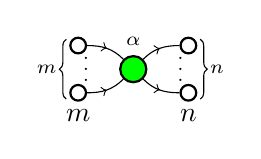
\begin{tikzpicture}
	\node [zxgreen,label={\scriptsize $\alpha$}] (v1) at (0,0) {};
	\node [zxopen] (v2) at (-0.7,0.3) {};
	\node [zxopen,label={[shift={(0,-0.6)}] $m$}] (v3) at (-0.7,-0.3) {};
	\node [zxopen] (v4) at (0.7,0.3) {};
	\node [zxopen,label={[shift={(0,-0.6)}] $n$}] (v5) at (0.7,-0.3) {};
	\node at (-0.6,0.1) {\scriptsize $\vdots$};
	\node at (0.6,0.1) {\scriptsize $\vdots$};
	\draw [->-]  (v2) to [out=0,in=135] (v1);
	\draw [->-] (v3) to [out=0,in=225] (v1);
	\draw [->-] (v1) to [out=45,in=180] (v4);
	\draw [->-] (v1) to [out=-45,in=180] (v5);
	\draw[decoration={brace,mirror,raise=2pt},decorate]
	(v2.north west) -- node [left=2pt] {\scriptsize $m$} (v3.south west); 
	\draw[decoration={brace,raise=2pt},decorate]
	(v4.north east) -- node [right=2pt] {\scriptsize $n$} (v5.south east); 	
\end{tikzpicture}
\]
\end{document}
